\section{Methods}

\subsection{Generating per-atom-type reference energies}
\paragraph{}
The two body component of the split unfolded reference energy consists of energy values for a set of atoms which are summed to determine the reference energy for any given amino acid or peptidomemetic. These energy values are obtained from an ensemble of a large number(above order $10^6$ for most atom types) of instances of that atom type in high resolution X-ray protein structures. These protein structures were obtained from the Top8000 benchmark set of high quality structures[ref-top8000], and was scored with Rosetta using a modified protocol that recorded every inter-atomic score term. These score terms were grouped by atom type and statistics were computed on the score distributions to provide expected energies for that atom type in a well-folded protein. We tested several different sets of atom types to determine which description of the atoms of an amino acid residue would best describe the inter-residue interactions expected for that residue. As two limit cases, we examined elemental types, wherein all atoms of the same element are alike, as well as unique atom types, where every atom from every residue type was assigned a different group. Intended to balance generalizability and goodness of fit, we also included the atom type sets used by Rosetta and by CHARMM[ref], as well as molecular mechanics atom types[ref?]. (what is the proper name for this atom type set?)

TABLE illustrating these atom types. I'm thinking a table at least containing GLY CA, ALA CA, ALA CB, and ALA C as rows. Elemental would group them all as C, MM/Rosetta would distinguish the CA+CB from C, Unique would distinguish all 4.

\paragraph{}
We considered different methods for obtaining an appropriate measure of centrality for the different distributions produced by these scoring terms, including the mean, median, mode, and Boltzmann-weighted average. Early testing showed that the distribution median was more robust across different atom types and performed better in sequence recovery trials, so we decided to use the median values in all further testing.


\subsection{Generating atom type distributions for NCAA's} 
\paragraph{}
In addition to the atom type energies derived from the top8000 structure benchmark as described above, a small number of mm atom types for NCAA types currently in Rosetta are not found in canonical amino acids, such as the various halogen atoms, and thus were not represented in the Top8000 data set. To obtain expected energy distributions for these atom types, we selected NCAA's containing those atom types, identified structurally and chemically similar canonical amino acids(e.g. trifluoro-leucine matched to leucine), and mutated all instances of the canonical analog in the top8000 benchmark to the NCAA of interest. We then resolved clashes produced by the differences between the residues using <XXX type of minimization?>, and used the score distributions resulting from iteration over all canonical analog positions in the top8000 to generate median energy values for each mm atom type not present in canonical amino acids.

TABLE of all the mm atom types covered, noting which ones are natural and which ones are mutated? Also note CAA analogs for NCAA's, and which atom types come from those NCAA's.

%%%Table sample code, adapt as needed
\begin{table}[h!]
  \begin{center}
    \caption{test table, please ignore}
    \label{table1}
    \pgfplotstabletypeset[
      multicolumn names,
      col sep=comma,
      display columns/0/.style={
        column name=$Value 1$
        column type={S},string type},
      every head row/.style={
        before row={\toprule},
        after row={
          \si{\ampere} & \st{\volt}\\
          \midrule}
      },
      every last row/.style={after row=\bottomrule},
      ]{NCAA_atom_types.csv}
    \end{center}
  \end{table}

FIGURE with one of the two body energy distributions for illustrative purposes. Makes sense to put it here, I think, rather than in results(since it's not a ``result'' per se)

\begin{figure}
  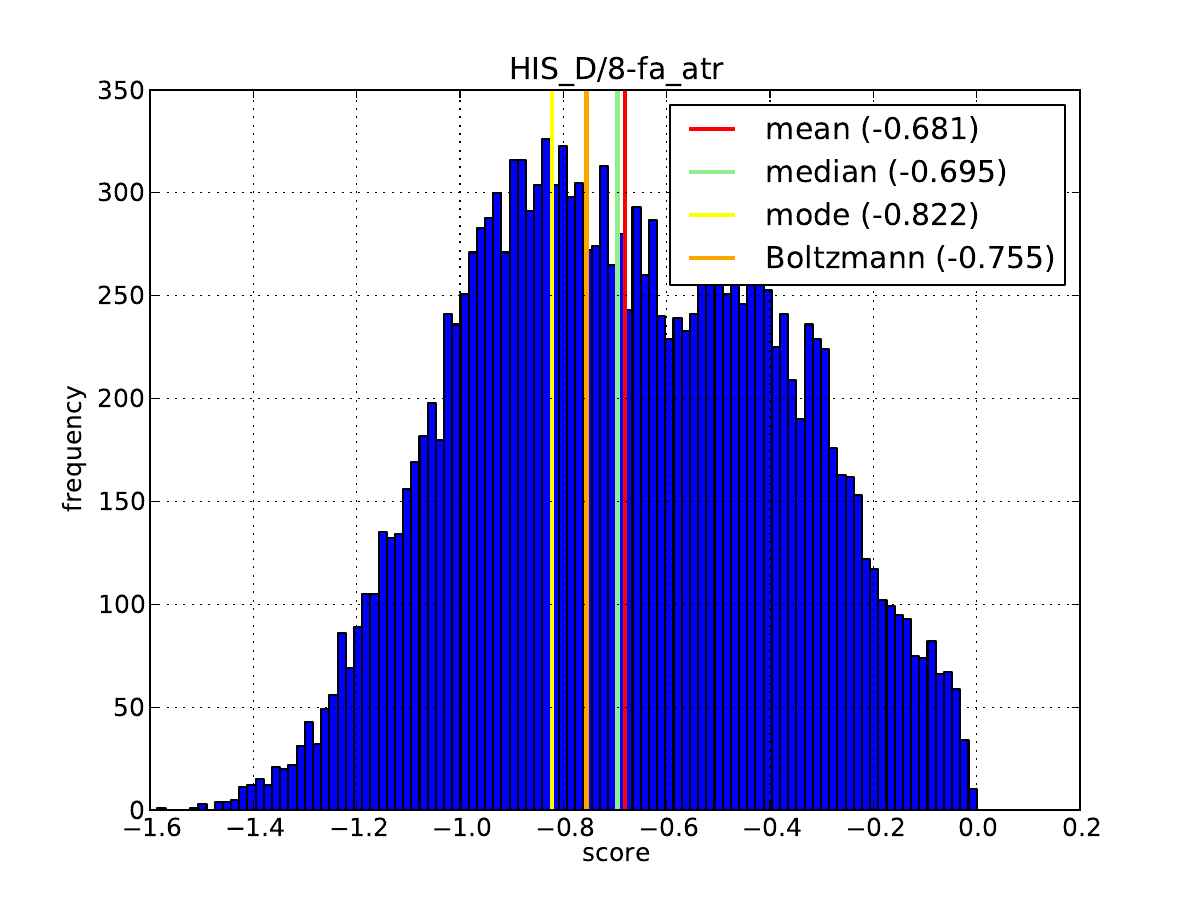
\includegraphics[width=\linewidth]{Figures/test.png}
  \caption{Example two body energy distribution.}
  \label{fig:tbaedist}
\end{figure}


\subsection{Formulation of the split unfolded reference energy}
\paragraph{}
Our split unfolded energy function is composed of two scoring terms in Rosetta, a one body and a two body component. During scoring, each of these terms is calculated separately for each residue in the protein, and then weighted and summed similar to each other Rosetta energy term. The formulation of the split unfolded reference energy for a protein is thus:

\begin{equation}
E_{\text{unfolded}} =  W_{1body} \sum_{i}^{n_{\text{res}}} E_{i,1body} +  W_{2body} \sum_{i}^{n_{\text{res}}} E_{i,2body}
\end{equation}

Where $W_{1body}$ is the weight placed on the one body term, $W_{2body}$ is the weight placed on the two body term, $E_{i,1body}$ is the one body component of the reference energy for residue $i$, and $E_{i,2body}$ is the two body component of the reference energy for residue $i$.

\subsection{Calculation of the two body energy term}
\paragraph{}
The two body component of the split unfolded energy consists of a sum of the energies of each constitutent atom. These atomic energies are calculated from instances of each atom type in the set used appearing in the top8000 data set of high-quality protein crystal structures, as described above. These values for each Rosetta score term calculated on a per-atom basis are stored in a lookup table, and per-residue two body unfolded energies are built dynamically as needed during runtime from these atom energy lookups. The two body split unfolded energy for the protein is calculated as follows:

\begin{equation}
E_{\text{2body}} = W_{2body} \sum_{i}^{n_{\text{res}}} \sum_{j}^{l_{\text{scoreterms}}} W_{j} \sum_{k}^{m_{\text{atoms}}} E_{k}
\end{equation}
Where $W_{two-body}$ is the weight value for the two body term, $n$ is the total number of residues, $l$ is the score terms $fa\_atr$, $fa\_rep$, $fa\_sol$, $fa\_elec$, $hbond$, and $fa\_dslf13$ for the $talaris2013$ scoring function and the score terms $fa\_atr$, $fa\_rep$, $fa\_elec$, $hbond$, and $fa\_dslf13$ for the $mm\_std$ scoring function, $W_{j}$ is the weight on score term $j$, $m$ is the number of atoms in the residue $i$, and $E_{k}$ is the energy of atom $k$ in the two body atom energy lookup table.


\subsection{Determining the single-body reference energy component}
\paragraph{}
For the one body component of the reference energy, representing the inherent energy of a given sidechain in an unfolded chain, we used a Rosetta simulation of acetylated and N-methylamidated versions of each monomer residue type to simulate the presence of neighboring residues in a chain. The backbone phi and psi angles of these residues were iterated in <?degree?> bins, with each bin angle minimized using Rosetta's <dfpmin?> minimizer to find local intra-residue energy minima. A low energy sidechain conformation was found for each backbone bin using rotamer repacking followed by minimization identical to that of the backbone. The lowest energy conformation among those sampled was taken as the ideal minimal monomeric conformation for each residue type, and their intra-residue energies recorded as the baseline energy introduced into a protein structure by designing that residue. This process was carried out using the intra-residue scoring terms for both the $talaris2013$ score function and the $mm\_std$ score function. For $talaris2013$, the intra-residue terms were <score terms>, while for $mm\_std$, the intra-residue terms were <other score terms>.

\paragraph{}
During runtime, the one body reference energy of a protein is determined by summing the values thus recorded for each residue type in it's sequence, which is then weighted and summed with the other score terms to produce the total energy of the protein.

METHOD FIGURE?


\subsection{How sequence recovery testing works}
\paragraph{}
To test the utility of our split unfolded reference energy for protein design, we used the Rosetta native sequence recovery benchmark protocol[ref?], which consists of a collection of <number> high-quality protein structures which are fully redesigned by Rosetta using a given scoring function to test its ability to recapitulate the native amino acid at each position as well as its ability to recapitulate the native amino acid frequencies, both of which indicate it's ability to design ``natural-like'' protein sequences for a given structure. While no benchmark set exists for the design of non-canonical residue types, performance on the canonical residue types should be indicative of performance on NCAA types as well, as these types are treated identically during runtime. <some more description of the protocol?>

To run the sequence recovery benchmark, the following command line was used:

<command line>



\subsection{Gridsearch how-done}
\paragraph{}
In addition to the generation of the energy terms for the one and two body split unfolded reference energy, as described above, there are also two weight parameters, $W_{2body}$ and $W_{1body}$, which can affect sequence recovery performance. Thus, optimization of these parameters is necessary in order to maximize design performance. 

\paragraph{}
As an initial step in optimizing these parameters, we used a simple grid-based search strategy, scanning combinations of $W_{2body}$ and $W_{1body}$ across the range of 1.0 to -1.0 for each weight(the typical range for Rosetta score term weights), in increments 0.05.


\subsection{optE description}
What optE did, how it did it. Complex, somewhat.

\subsection{optE optimization setup}
What exactly we did with optE to produce the results we did. May want to only have this for the revamped optE.

\subsection{new-optE description}
What it now does.
